\documentclass[1p]{elsarticle_modified}
%\bibliographystyle{elsarticle-num}

%\usepackage[colorlinks]{hyperref}
%\usepackage{abbrmath_seonhwa} %\Abb, \Ascr, \Acal ,\Abf, \Afrak
\usepackage{amsfonts}
\usepackage{amssymb}
\usepackage{amsmath}
\usepackage{amsthm}
\usepackage{scalefnt}
\usepackage{amsbsy}
\usepackage{kotex}
\usepackage{caption}
\usepackage{subfig}
\usepackage{color}
\usepackage{graphicx}
\usepackage{xcolor} %% white, black, red, green, blue, cyan, magenta, yellow
\usepackage{float}
\usepackage{setspace}
\usepackage{hyperref}

\usepackage{tikz}
\usetikzlibrary{arrows}

\usepackage{multirow}
\usepackage{array} % fixed length table
\usepackage{hhline}

%%%%%%%%%%%%%%%%%%%%%
\makeatletter
\renewcommand*\env@matrix[1][\arraystretch]{%
	\edef\arraystretch{#1}%
	\hskip -\arraycolsep
	\let\@ifnextchar\new@ifnextchar
	\array{*\c@MaxMatrixCols c}}
\makeatother %https://tex.stackexchange.com/questions/14071/how-can-i-increase-the-line-spacing-in-a-matrix
%%%%%%%%%%%%%%%

\usepackage[normalem]{ulem}

\newcommand{\msout}[1]{\ifmmode\text{\sout{\ensuremath{#1}}}\else\sout{#1}\fi}
%SOURCE: \msout is \stkout macro in https://tex.stackexchange.com/questions/20609/strikeout-in-math-mode

\newcommand{\cancel}[1]{
	\ifmmode
	{\color{red}\msout{#1}}
	\else
	{\color{red}\sout{#1}}
	\fi
}

\newcommand{\add}[1]{
	{\color{blue}\uwave{#1}}
}

\newcommand{\replace}[2]{
	\ifmmode
	{\color{red}\msout{#1}}{\color{blue}\uwave{#2}}
	\else
	{\color{red}\sout{#1}}{\color{blue}\uwave{#2}}
	\fi
}

\newcommand{\Sol}{\mathcal{S}} %segment
\newcommand{\D}{D} %diagram
\newcommand{\A}{\mathcal{A}} %arc


%%%%%%%%%%%%%%%%%%%%%%%%%%%%%5 test

\def\sl{\operatorname{\textup{SL}}(2,\Cbb)}
\def\psl{\operatorname{\textup{PSL}}(2,\Cbb)}
\def\quan{\mkern 1mu \triangleright \mkern 1mu}

\theoremstyle{definition}
\newtheorem{thm}{Theorem}[section]
\newtheorem{prop}[thm]{Proposition}
\newtheorem{lem}[thm]{Lemma}
\newtheorem{ques}[thm]{Question}
\newtheorem{cor}[thm]{Corollary}
\newtheorem{defn}[thm]{Definition}
\newtheorem{exam}[thm]{Example}
\newtheorem{rmk}[thm]{Remark}
\newtheorem{alg}[thm]{Algorithm}

\newcommand{\I}{\sqrt{-1}}
\begin{document}

%\begin{frontmatter}
%
%\title{Boundary parabolic representations of knots up to 8 crossings}
%
%%% Group authors per affiliation:
%\author{Yunhi Cho} 
%\address{Department of Mathematics, University of Seoul, Seoul, Korea}
%\ead{yhcho@uos.ac.kr}
%
%
%\author{Seonhwa Kim} %\fnref{s_kim}}
%\address{Center for Geometry and Physics, Institute for Basic Science, Pohang, 37673, Korea}
%\ead{ryeona17@ibs.re.kr}
%
%\author{Hyuk Kim}
%\address{Department of Mathematical Sciences, Seoul National University, Seoul 08826, Korea}
%\ead{hyukkim@snu.ac.kr}
%
%\author{Seokbeom Yoon}
%\address{Department of Mathematical Sciences, Seoul National University, Seoul, 08826,  Korea}
%\ead{sbyoon15@snu.ac.kr}
%
%\begin{abstract}
%We find all boundary parabolic representation of knots up to 8 crossings.
%
%\end{abstract}
%\begin{keyword}
%    \MSC[2010] 57M25 
%\end{keyword}
%
%\end{frontmatter}

%\linenumbers
%\tableofcontents
%
\newcommand\colored[1]{\textcolor{white}{\rule[-0.35ex]{0.8em}{1.4ex}}\kern-0.8em\color{red} #1}%
%\newcommand\colored[1]{\textcolor{white}{ #1}\kern-2.17ex	\textcolor{white}{ #1}\kern-1.81ex	\textcolor{white}{ #1}\kern-2.15ex\color{red}#1	}

{\Large $\underline{11n_{131}~(K11n_{131})}$}

\setlength{\tabcolsep}{10pt}
\renewcommand{\arraystretch}{1.6}
\vspace{1cm}\begin{tabular}{m{100pt}>{\centering\arraybackslash}m{274pt}}
\multirow{5}{120pt}{
	\centering
	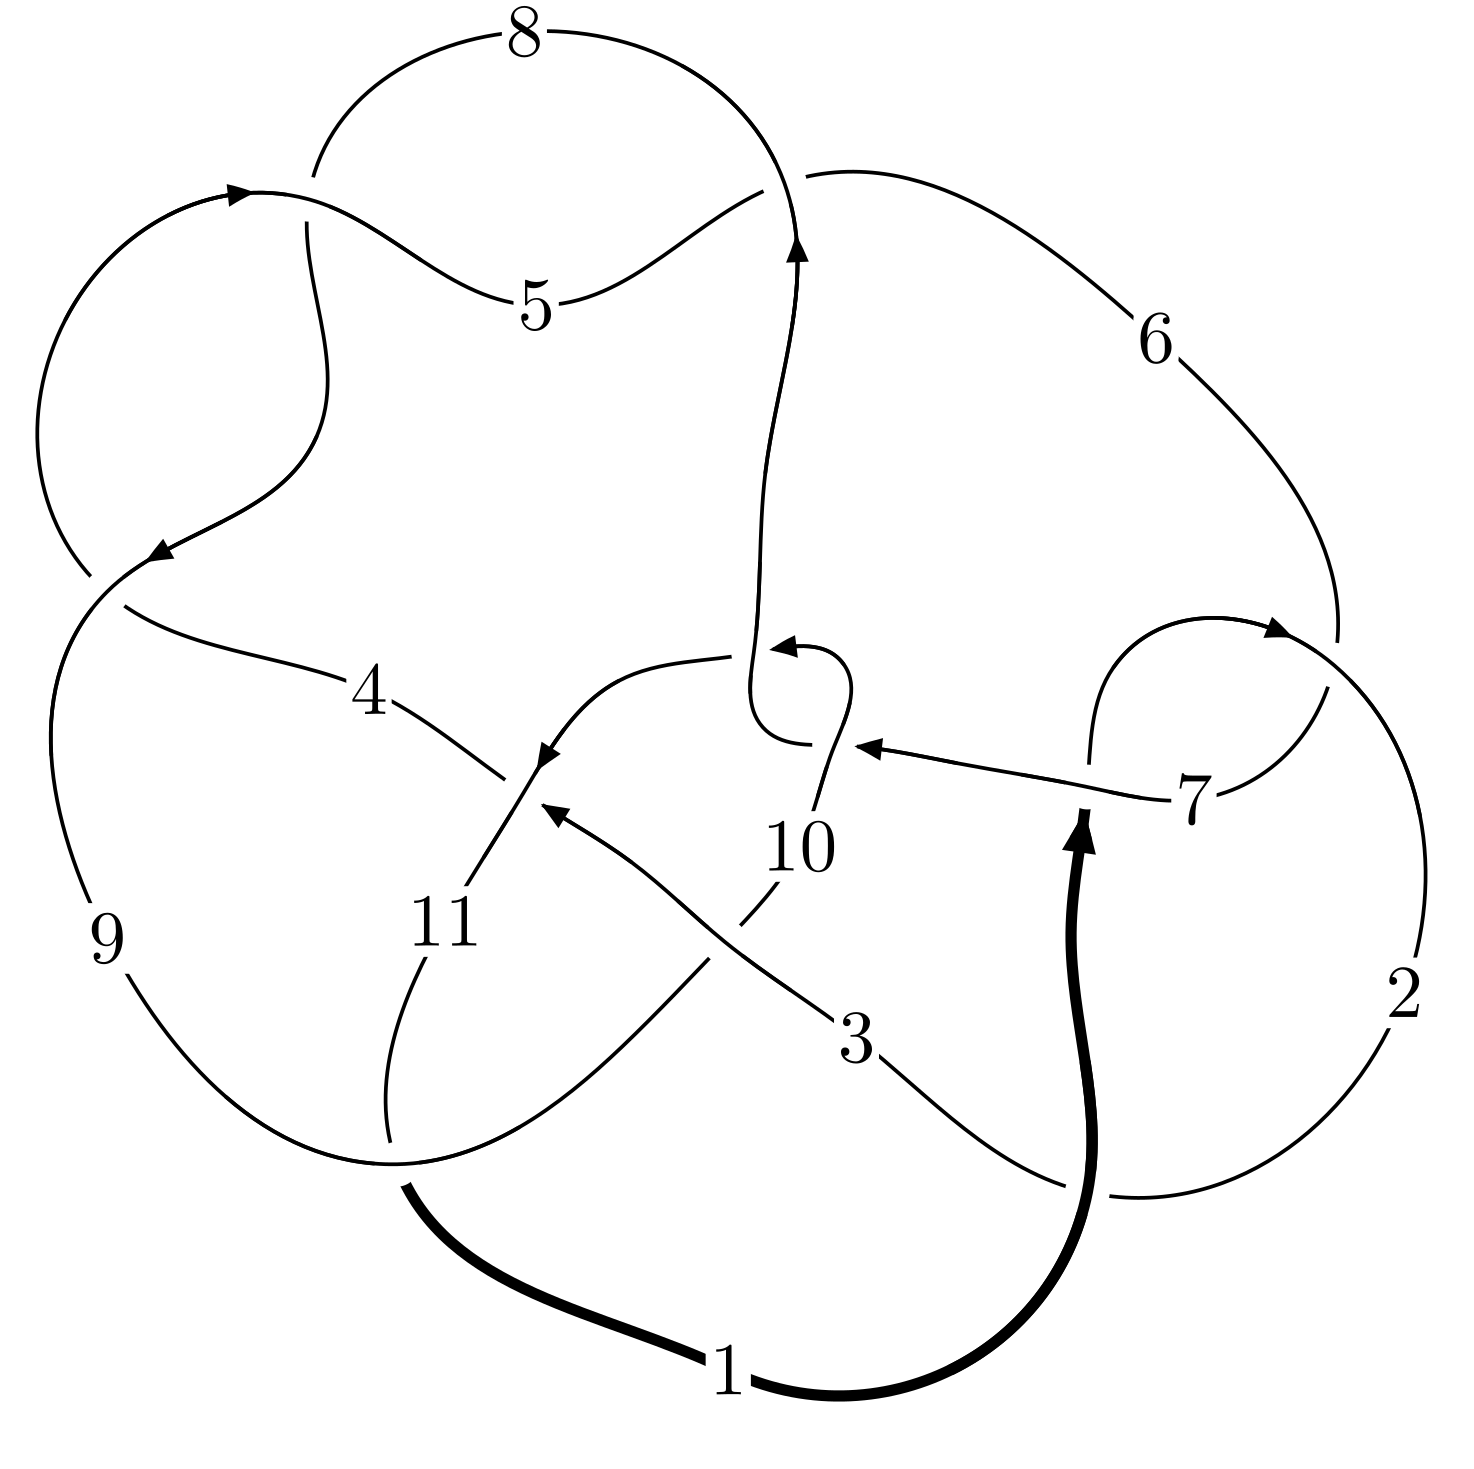
\includegraphics[width=112pt]{../../../GIT/diagram.site/Diagrams/png/747_11n_131.png}\\
\ \ \ A knot diagram\footnotemark}&
\allowdisplaybreaks
\textbf{Linearized knot diagam} \\
\cline{2-2}
 &
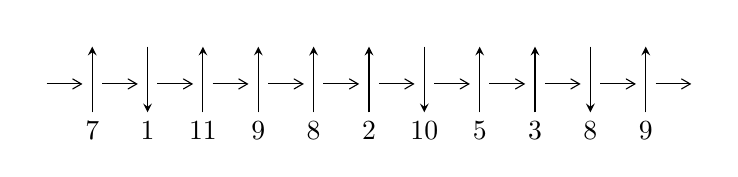
\begin{tikzpicture}[x=20pt, y=17pt]
	% nodes
	\node (C0) at (0, 0) {};
	\node (C1) at (1, 0) {};
	\node (C1U) at (1, +1) {};
	\node (C1D) at (1, -1) {7};

	\node (C2) at (2, 0) {};
	\node (C2U) at (2, +1) {};
	\node (C2D) at (2, -1) {1};

	\node (C3) at (3, 0) {};
	\node (C3U) at (3, +1) {};
	\node (C3D) at (3, -1) {11};

	\node (C4) at (4, 0) {};
	\node (C4U) at (4, +1) {};
	\node (C4D) at (4, -1) {9};

	\node (C5) at (5, 0) {};
	\node (C5U) at (5, +1) {};
	\node (C5D) at (5, -1) {8};

	\node (C6) at (6, 0) {};
	\node (C6U) at (6, +1) {};
	\node (C6D) at (6, -1) {2};

	\node (C7) at (7, 0) {};
	\node (C7U) at (7, +1) {};
	\node (C7D) at (7, -1) {10};

	\node (C8) at (8, 0) {};
	\node (C8U) at (8, +1) {};
	\node (C8D) at (8, -1) {5};

	\node (C9) at (9, 0) {};
	\node (C9U) at (9, +1) {};
	\node (C9D) at (9, -1) {3};

	\node (C10) at (10, 0) {};
	\node (C10U) at (10, +1) {};
	\node (C10D) at (10, -1) {8};

	\node (C11) at (11, 0) {};
	\node (C11U) at (11, +1) {};
	\node (C11D) at (11, -1) {9};
	\node (C12) at (12, 0) {};

	% arrows
	\draw[->,>={angle 60}]
	(C0) edge (C1) (C1) edge (C2) (C2) edge (C3) (C3) edge (C4) (C4) edge (C5) (C5) edge (C6) (C6) edge (C7) (C7) edge (C8) (C8) edge (C9) (C9) edge (C10) (C10) edge (C11) (C11) edge (C12) ;	\draw[->,>=stealth]
	(C1D) edge (C1U) (C2U) edge (C2D) (C3D) edge (C3U) (C4D) edge (C4U) (C5D) edge (C5U) (C6D) edge (C6U) (C7U) edge (C7D) (C8D) edge (C8U) (C9D) edge (C9U) (C10U) edge (C10D) (C11D) edge (C11U) ;
	\end{tikzpicture} \\
\hhline{~~} \\& 
\textbf{Solving Sequence} \\ \cline{2-2} 
 &
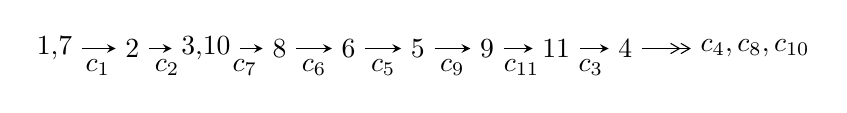
\begin{tikzpicture}[x=25pt, y=7pt]
	% node
	\node (A0) at (-1/8, 0) {1,7};
	\node (A1) at (1, 0) {2};
	\node (A2) at (33/16, 0) {3,10};
	\node (A3) at (25/8, 0) {8};
	\node (A4) at (33/8, 0) {6};
	\node (A5) at (41/8, 0) {5};
	\node (A6) at (49/8, 0) {9};
	\node (A7) at (57/8, 0) {11};
	\node (A8) at (65/8, 0) {4};
	\node (C1) at (1/2, -1) {$c_{1}$};
	\node (C2) at (3/2, -1) {$c_{2}$};
	\node (C3) at (21/8, -1) {$c_{7}$};
	\node (C4) at (29/8, -1) {$c_{6}$};
	\node (C5) at (37/8, -1) {$c_{5}$};
	\node (C6) at (45/8, -1) {$c_{9}$};
	\node (C7) at (53/8, -1) {$c_{11}$};
	\node (C8) at (61/8, -1) {$c_{3}$};
	\node (A9) at (10, 0) {$c_{4},c_{8},c_{10}$};

	% edge
	\draw[->,>=stealth]	
	(A0) edge (A1) (A1) edge (A2) (A2) edge (A3) (A3) edge (A4) (A4) edge (A5) (A5) edge (A6) (A6) edge (A7) (A7) edge (A8) ;
	\draw[->>,>={angle 60}]	
	(A8) edge (A9);
\end{tikzpicture} \\ 

\end{tabular} \\

\footnotetext{
The image of knot diagram is generated by the software ``\textbf{Draw programme}" developed by Andrew Bartholomew(\url{http://www.layer8.co.uk/maths/draw/index.htm\#Running-draw}), where we modified some parts for our purpose(\url{https://github.com/CATsTAILs/LinksPainter}).
}\phantom \\ \newline 
\centering \textbf{Ideals for irreducible components\footnotemark of $X_{\text{par}}$} 
 
\begin{align*}
I^u_{1}&=\langle 
-9.69653\times10^{36} u^{43}+1.93812\times10^{38} u^{42}+\cdots+1.36546\times10^{39} b+1.44554\times10^{39},\\
\phantom{I^u_{1}}&\phantom{= \langle  }2.34671\times10^{40} u^{43}-2.31254\times10^{39} u^{42}+\cdots+2.59437\times10^{40} a+1.06428\times10^{41},\;u^{44}+8 u^{42}+\cdots+28 u+19\rangle \\
I^u_{2}&=\langle 
- u^{10}-2 u^9-3 u^8-5 u^7-6 u^6-10 u^5-9 u^4-8 u^3-9 u^2+b-4 u-4,\\
\phantom{I^u_{2}}&\phantom{= \langle  }- u^9- u^8-2 u^7-2 u^6-3 u^5-5 u^4-2 u^3-3 u^2+a- u-2,\\
\phantom{I^u_{2}}&\phantom{= \langle  }u^{11}+u^{10}+3 u^9+3 u^8+5 u^7+7 u^6+5 u^5+8 u^4+3 u^3+5 u^2+u+1\rangle \\
\\
\end{align*}
\raggedright * 2 irreducible components of $\dim_{\mathbb{C}}=0$, with total 55 representations.\\
\footnotetext{All coefficients of polynomials are rational numbers. But the coefficients are sometimes approximated in decimal forms when there is not enough margin.}
\newpage
\renewcommand{\arraystretch}{1}
\centering \section*{I. $I^u_{1}= \langle -9.70\times10^{36} u^{43}+1.94\times10^{38} u^{42}+\cdots+1.37\times10^{39} b+1.45\times10^{39},\;2.35\times10^{40} u^{43}-2.31\times10^{39} u^{42}+\cdots+2.59\times10^{40} a+1.06\times10^{41},\;u^{44}+8 u^{42}+\cdots+28 u+19 \rangle$}
\flushleft \textbf{(i) Arc colorings}\\
\begin{tabular}{m{7pt} m{180pt} m{7pt} m{180pt} }
\flushright $a_{1}=$&$\begin{pmatrix}1\\0\end{pmatrix}$ \\
\flushright $a_{7}=$&$\begin{pmatrix}0\\u\end{pmatrix}$ \\
\flushright $a_{2}=$&$\begin{pmatrix}1\\- u^2\end{pmatrix}$ \\
\flushright $a_{3}=$&$\begin{pmatrix}u^2+1\\- u^2\end{pmatrix}$ \\
\flushright $a_{10}=$&$\begin{pmatrix}-0.904540 u^{43}+0.0891368 u^{42}+\cdots-28.1734 u-4.10227\\0.00710130 u^{43}-0.141939 u^{42}+\cdots-5.47040 u-1.05865\end{pmatrix}$ \\
\flushright $a_{8}=$&$\begin{pmatrix}0.129802 u^{43}-0.616286 u^{42}+\cdots-13.9864 u-18.1892\\-0.112721 u^{43}+0.238849 u^{42}+\cdots-2.68255 u+7.40994\end{pmatrix}$ \\
\flushright $a_{6}=$&$\begin{pmatrix}- u\\u^3+u\end{pmatrix}$ \\
\flushright $a_{5}=$&$\begin{pmatrix}0.855694 u^{43}+0.294688 u^{42}+\cdots+42.8937 u+18.2259\\-0.198202 u^{43}-0.0959296 u^{42}+\cdots-8.51213 u-7.37608\end{pmatrix}$ \\
\flushright $a_{9}=$&$\begin{pmatrix}-1.12405 u^{43}-0.0401899 u^{42}+\cdots-35.9422 u-8.61657\\-0.406276 u^{43}+0.227899 u^{42}+\cdots-10.7610 u+3.51106\end{pmatrix}$ \\
\flushright $a_{11}=$&$\begin{pmatrix}-0.232879 u^{43}+0.618756 u^{42}+\cdots+6.55564 u+18.5444\\0.0121303 u^{43}+0.0705266 u^{42}+\cdots+6.59355 u+5.72029\end{pmatrix}$ \\
\flushright $a_{4}=$&$\begin{pmatrix}-0.925125 u^{43}+0.652168 u^{42}+\cdots-16.2508 u+7.52727\\0.107850 u^{43}+0.505554 u^{42}+\cdots+18.8829 u+20.6647\end{pmatrix}$\\ \flushright $a_{4}=$&$\begin{pmatrix}-0.925125 u^{43}+0.652168 u^{42}+\cdots-16.2508 u+7.52727\\0.107850 u^{43}+0.505554 u^{42}+\cdots+18.8829 u+20.6647\end{pmatrix}$\\&\end{tabular}
\flushleft \textbf{(ii) Obstruction class $= -1$}\\~\\
\flushleft \textbf{(iii) Cusp Shapes $= -0.830501 u^{43}-1.97049 u^{42}+\cdots-84.2334 u-62.6447$}\\~\\
\newpage\renewcommand{\arraystretch}{1}
\flushleft \textbf{(iv) u-Polynomials at the component}\newline \\
\begin{tabular}{m{50pt}|m{274pt}}
Crossings & \hspace{64pt}u-Polynomials at each crossing \\
\hline $$\begin{aligned}c_{1},c_{6}\end{aligned}$$&$\begin{aligned}
&u^{44}+8 u^{42}+\cdots+28 u+19
\end{aligned}$\\
\hline $$\begin{aligned}c_{2}\end{aligned}$$&$\begin{aligned}
&u^{44}+16 u^{43}+\cdots+3928 u+361
\end{aligned}$\\
\hline $$\begin{aligned}c_{3}\end{aligned}$$&$\begin{aligned}
&u^{44}+4 u^{43}+\cdots+13 u+1
\end{aligned}$\\
\hline $$\begin{aligned}c_{4},c_{5},c_{8}\end{aligned}$$&$\begin{aligned}
&u^{44}+2 u^{43}+\cdots-11 u-1
\end{aligned}$\\
\hline $$\begin{aligned}c_{7},c_{10}\end{aligned}$$&$\begin{aligned}
&u^{44}+u^{43}+\cdots-41 u+11
\end{aligned}$\\
\hline $$\begin{aligned}c_{9}\end{aligned}$$&$\begin{aligned}
&u^{44}- u^{43}+\cdots-14 u-1
\end{aligned}$\\
\hline $$\begin{aligned}c_{11}\end{aligned}$$&$\begin{aligned}
&u^{44}+2 u^{43}+\cdots+12 u-1
\end{aligned}$\\
\hline
\end{tabular}\\~\\
\newpage\renewcommand{\arraystretch}{1}
\flushleft \textbf{(v) Riley Polynomials at the component}\newline \\
\begin{tabular}{m{50pt}|m{274pt}}
Crossings & \hspace{64pt}Riley Polynomials at each crossing \\
\hline $$\begin{aligned}c_{1},c_{6}\end{aligned}$$&$\begin{aligned}
&y^{44}+16 y^{43}+\cdots+3928 y+361
\end{aligned}$\\
\hline $$\begin{aligned}c_{2}\end{aligned}$$&$\begin{aligned}
&y^{44}+24 y^{43}+\cdots-363932 y+130321
\end{aligned}$\\
\hline $$\begin{aligned}c_{3}\end{aligned}$$&$\begin{aligned}
&y^{44}-42 y^{43}+\cdots-5 y+1
\end{aligned}$\\
\hline $$\begin{aligned}c_{4},c_{5},c_{8}\end{aligned}$$&$\begin{aligned}
&y^{44}+12 y^{43}+\cdots-37 y+1
\end{aligned}$\\
\hline $$\begin{aligned}c_{7},c_{10}\end{aligned}$$&$\begin{aligned}
&y^{44}-15 y^{43}+\cdots-2869 y+121
\end{aligned}$\\
\hline $$\begin{aligned}c_{9}\end{aligned}$$&$\begin{aligned}
&y^{44}+7 y^{43}+\cdots-54 y+1
\end{aligned}$\\
\hline $$\begin{aligned}c_{11}\end{aligned}$$&$\begin{aligned}
&y^{44}-38 y^{43}+\cdots-96 y+1
\end{aligned}$\\
\hline
\end{tabular}\\~\\
\newpage\flushleft \textbf{(vi) Complex Volumes and Cusp Shapes}
$$\begin{array}{c|c|c}  
\text{Solutions to }I^u_{1}& \I (\text{vol} + \sqrt{-1}CS) & \text{Cusp shape}\\
 \hline 
\begin{aligned}
u &= -0.553611 + 0.824772 I \\
a &= \phantom{-}0.447859 + 1.150180 I \\
b &= -1.49583 - 0.39989 I\end{aligned}
 & -3.21451 - 2.15595 I & \phantom{-}1.07743 + 2.96858 I \\ \hline\begin{aligned}
u &= -0.553611 - 0.824772 I \\
a &= \phantom{-}0.447859 - 1.150180 I \\
b &= -1.49583 + 0.39989 I\end{aligned}
 & -3.21451 + 2.15595 I & \phantom{-}1.07743 - 2.96858 I \\ \hline\begin{aligned}
u &= \phantom{-}0.691309 + 0.811314 I \\
a &= -1.341520 + 0.125641 I \\
b &= -0.247744 + 0.790756 I\end{aligned}
 & \phantom{-}4.27651 - 0.41832 I & \phantom{-}5.68762 - 0.89780 I \\ \hline\begin{aligned}
u &= \phantom{-}0.691309 - 0.811314 I \\
a &= -1.341520 - 0.125641 I \\
b &= -0.247744 - 0.790756 I\end{aligned}
 & \phantom{-}4.27651 + 0.41832 I & \phantom{-}5.68762 + 0.89780 I \\ \hline\begin{aligned}
u &= -0.749080 + 0.765100 I \\
a &= \phantom{-}0.129349 - 1.222590 I \\
b &= \phantom{-}0.61597 + 1.72869 I\end{aligned}
 & \phantom{-}5.60971 + 1.02097 I & \phantom{-}7.05881 + 0.21382 I \\ \hline\begin{aligned}
u &= -0.749080 - 0.765100 I \\
a &= \phantom{-}0.129349 + 1.222590 I \\
b &= \phantom{-}0.61597 - 1.72869 I\end{aligned}
 & \phantom{-}5.60971 - 1.02097 I & \phantom{-}7.05881 - 0.21382 I \\ \hline\begin{aligned}
u &= -0.358331 + 0.841835 I \\
a &= \phantom{-}0.73681 + 1.63006 I \\
b &= -0.800323 - 0.656423 I\end{aligned}
 & -4.31132 - 1.52913 I & \phantom{-}4.89215 + 5.65142 I \\ \hline\begin{aligned}
u &= -0.358331 - 0.841835 I \\
a &= \phantom{-}0.73681 - 1.63006 I \\
b &= -0.800323 + 0.656423 I\end{aligned}
 & -4.31132 + 1.52913 I & \phantom{-}4.89215 - 5.65142 I \\ \hline\begin{aligned}
u &= \phantom{-}0.724746 + 0.501149 I \\
a &= \phantom{-}0.790041 + 0.280445 I \\
b &= \phantom{-}0.212674 - 0.438603 I\end{aligned}
 & \phantom{-}1.31409 + 0.60593 I & \phantom{-}8.59743 - 3.14385 I \\ \hline\begin{aligned}
u &= \phantom{-}0.724746 - 0.501149 I \\
a &= \phantom{-}0.790041 - 0.280445 I \\
b &= \phantom{-}0.212674 + 0.438603 I\end{aligned}
 & \phantom{-}1.31409 - 0.60593 I & \phantom{-}8.59743 + 3.14385 I\\
 \hline 
 \end{array}$$\newpage$$\begin{array}{c|c|c}  
\text{Solutions to }I^u_{1}& \I (\text{vol} + \sqrt{-1}CS) & \text{Cusp shape}\\
 \hline 
\begin{aligned}
u &= \phantom{-}0.672004 + 0.909211 I \\
a &= -0.118766 + 1.200990 I \\
b &= \phantom{-}0.67880 - 1.94511 I\end{aligned}
 & \phantom{-}3.96994 + 5.67612 I & \phantom{-}4.70172 - 5.28440 I \\ \hline\begin{aligned}
u &= \phantom{-}0.672004 - 0.909211 I \\
a &= -0.118766 - 1.200990 I \\
b &= \phantom{-}0.67880 + 1.94511 I\end{aligned}
 & \phantom{-}3.96994 - 5.67612 I & \phantom{-}4.70172 + 5.28440 I \\ \hline\begin{aligned}
u &= -0.305333 + 1.097040 I \\
a &= \phantom{-}0.502841 + 0.752892 I \\
b &= -0.431064 - 0.191810 I\end{aligned}
 & -3.64801 - 0.66413 I & -0.67434 - 1.82360 I \\ \hline\begin{aligned}
u &= -0.305333 - 1.097040 I \\
a &= \phantom{-}0.502841 - 0.752892 I \\
b &= -0.431064 + 0.191810 I\end{aligned}
 & -3.64801 + 0.66413 I & -0.67434 + 1.82360 I \\ \hline\begin{aligned}
u &= -0.724813 + 0.904533 I \\
a &= -0.048082 - 0.448492 I \\
b &= \phantom{-}1.168590 - 0.034882 I\end{aligned}
 & -4.81373 - 2.81453 I & \phantom{-}7.83387 + 2.63389 I \\ \hline\begin{aligned}
u &= -0.724813 - 0.904533 I \\
a &= -0.048082 + 0.448492 I \\
b &= \phantom{-}1.168590 + 0.034882 I\end{aligned}
 & -4.81373 + 2.81453 I & \phantom{-}7.83387 - 2.63389 I \\ \hline\begin{aligned}
u &= -0.155660 + 0.819694 I \\
a &= -0.50119 - 1.50907 I \\
b &= -0.837138 + 0.913868 I\end{aligned}
 & -8.09531 - 0.68903 I & -3.33839 - 2.14717 I \\ \hline\begin{aligned}
u &= -0.155660 - 0.819694 I \\
a &= -0.50119 + 1.50907 I \\
b &= -0.837138 - 0.913868 I\end{aligned}
 & -8.09531 + 0.68903 I & -3.33839 + 2.14717 I \\ \hline\begin{aligned}
u &= -1.035790 + 0.563745 I \\
a &= -1.135220 + 0.231350 I \\
b &= \phantom{-}0.457170 - 1.082790 I\end{aligned}
 & \phantom{-}4.92535 + 7.92322 I & \phantom{-}5.81282 - 4.97707 I \\ \hline\begin{aligned}
u &= -1.035790 - 0.563745 I \\
a &= -1.135220 - 0.231350 I \\
b &= \phantom{-}0.457170 + 1.082790 I\end{aligned}
 & \phantom{-}4.92535 - 7.92322 I & \phantom{-}5.81282 + 4.97707 I\\
 \hline 
 \end{array}$$\newpage$$\begin{array}{c|c|c}  
\text{Solutions to }I^u_{1}& \I (\text{vol} + \sqrt{-1}CS) & \text{Cusp shape}\\
 \hline 
\begin{aligned}
u &= -0.702097 + 0.948685 I \\
a &= -1.230740 + 0.211924 I \\
b &= -0.165846 - 1.175810 I\end{aligned}
 & \phantom{-}5.04402 - 6.54331 I & \phantom{-}5.65027 + 5.81604 I \\ \hline\begin{aligned}
u &= -0.702097 - 0.948685 I \\
a &= -1.230740 - 0.211924 I \\
b &= -0.165846 + 1.175810 I\end{aligned}
 & \phantom{-}5.04402 + 6.54331 I & \phantom{-}5.65027 - 5.81604 I \\ \hline\begin{aligned}
u &= \phantom{-}0.191318 + 0.786546 I \\
a &= -0.321704 + 0.371146 I \\
b &= \phantom{-}2.20155 - 0.83164 I\end{aligned}
 & \phantom{-}1.02150 - 1.91904 I & -0.873774 - 0.783296 I \\ \hline\begin{aligned}
u &= \phantom{-}0.191318 - 0.786546 I \\
a &= -0.321704 - 0.371146 I \\
b &= \phantom{-}2.20155 + 0.83164 I\end{aligned}
 & \phantom{-}1.02150 + 1.91904 I & -0.873774 + 0.783296 I \\ \hline\begin{aligned}
u &= -0.525867 + 1.092400 I \\
a &= -0.400089 + 1.030590 I \\
b &= -1.09956 - 1.76264 I\end{aligned}
 & -2.17094 - 6.60740 I & -0.69632 + 10.88929 I \\ \hline\begin{aligned}
u &= -0.525867 - 1.092400 I \\
a &= -0.400089 - 1.030590 I \\
b &= -1.09956 + 1.76264 I\end{aligned}
 & -2.17094 + 6.60740 I & -0.69632 - 10.88929 I \\ \hline\begin{aligned}
u &= \phantom{-}0.769126\phantom{ +0.000000I} \\
a &= \phantom{-}0.807876\phantom{ +0.000000I} \\
b &= \phantom{-}0.267033\phantom{ +0.000000I}\end{aligned}
 & \phantom{-}1.54727\phantom{ +0.000000I} & \phantom{-}4.67400\phantom{ +0.000000I} \\ \hline\begin{aligned}
u &= \phantom{-}1.004830 + 0.721198 I \\
a &= -0.817876 - 0.261435 I \\
b &= \phantom{-}0.420704 + 1.060050 I\end{aligned}
 & \phantom{-}5.67789 - 0.23429 I & \phantom{-}7.33450 + 1.57451 I \\ \hline\begin{aligned}
u &= \phantom{-}1.004830 - 0.721198 I \\
a &= -0.817876 + 0.261435 I \\
b &= \phantom{-}0.420704 - 1.060050 I\end{aligned}
 & \phantom{-}5.67789 + 0.23429 I & \phantom{-}7.33450 - 1.57451 I \\ \hline\begin{aligned}
u &= -0.038388 + 0.751954 I \\
a &= \phantom{-}1.43109 + 0.27249 I \\
b &= \phantom{-}1.141290 + 0.618112 I\end{aligned}
 & \phantom{-}0.97471 + 2.65784 I & -0.64848 - 4.81672 I\\
 \hline 
 \end{array}$$\newpage$$\begin{array}{c|c|c}  
\text{Solutions to }I^u_{1}& \I (\text{vol} + \sqrt{-1}CS) & \text{Cusp shape}\\
 \hline 
\begin{aligned}
u &= -0.038388 - 0.751954 I \\
a &= \phantom{-}1.43109 - 0.27249 I \\
b &= \phantom{-}1.141290 - 0.618112 I\end{aligned}
 & \phantom{-}0.97471 - 2.65784 I & -0.64848 + 4.81672 I \\ \hline\begin{aligned}
u &= \phantom{-}0.489616 + 1.163080 I \\
a &= \phantom{-}0.051203 - 0.505529 I \\
b &= -0.89249 + 1.30630 I\end{aligned}
 & -1.75776 + 4.42520 I & \phantom{-0.000000 } 0. - 2.66999 I \\ \hline\begin{aligned}
u &= \phantom{-}0.489616 - 1.163080 I \\
a &= \phantom{-}0.051203 + 0.505529 I \\
b &= -0.89249 - 1.30630 I\end{aligned}
 & -1.75776 - 4.42520 I & \phantom{-0.000000 -}0. + 2.66999 I \\ \hline\begin{aligned}
u &= -0.634927 + 0.276340 I \\
a &= \phantom{-}1.29507 - 0.74684 I \\
b &= -0.103239 + 0.918524 I\end{aligned}
 & \phantom{-}0.09044 + 2.10677 I & \phantom{-}3.45567 - 5.29032 I \\ \hline\begin{aligned}
u &= -0.634927 - 0.276340 I \\
a &= \phantom{-}1.29507 + 0.74684 I \\
b &= -0.103239 - 0.918524 I\end{aligned}
 & \phantom{-}0.09044 - 2.10677 I & \phantom{-}3.45567 + 5.29032 I \\ \hline\begin{aligned}
u &= \phantom{-}0.725736 + 1.115000 I \\
a &= \phantom{-}0.122771 - 0.880273 I \\
b &= -0.87157 + 1.15445 I\end{aligned}
 & -0.55823 + 5.04012 I & \phantom{-}8.95344 - 5.95960 I \\ \hline\begin{aligned}
u &= \phantom{-}0.725736 - 1.115000 I \\
a &= \phantom{-}0.122771 + 0.880273 I \\
b &= -0.87157 - 1.15445 I\end{aligned}
 & -0.55823 - 5.04012 I & \phantom{-}8.95344 + 5.95960 I \\ \hline\begin{aligned}
u &= \phantom{-}1.33218\phantom{ +0.000000I} \\
a &= \phantom{-}0.419650\phantom{ +0.000000I} \\
b &= -0.343484\phantom{ +0.000000I}\end{aligned}
 & \phantom{-}2.55385\phantom{ +0.000000I} & -14.8810\phantom{ +0.000000I} \\ \hline\begin{aligned}
u &= \phantom{-}0.801504 + 1.072620 I \\
a &= \phantom{-}0.171221 + 0.993803 I \\
b &= \phantom{-}1.18028 - 1.27689 I\end{aligned}
 & \phantom{-}4.52542 + 6.79447 I & \phantom{-}5.00000 - 4.75364 I \\ \hline\begin{aligned}
u &= \phantom{-}0.801504 - 1.072620 I \\
a &= \phantom{-}0.171221 - 0.993803 I \\
b &= \phantom{-}1.18028 + 1.27689 I\end{aligned}
 & \phantom{-}4.52542 - 6.79447 I & \phantom{-}5.00000 + 4.75364 I\\
 \hline 
 \end{array}$$\newpage$$\begin{array}{c|c|c}  
\text{Solutions to }I^u_{1}& \I (\text{vol} + \sqrt{-1}CS) & \text{Cusp shape}\\
 \hline 
\begin{aligned}
u &= -0.748515 + 1.151140 I \\
a &= \phantom{-}0.050409 - 1.131160 I \\
b &= \phantom{-}1.37231 + 1.59702 I\end{aligned}
 & \phantom{-}3.0688 - 14.3723 I & \phantom{-0.000000 -}0. + 8.23244 I \\ \hline\begin{aligned}
u &= -0.748515 - 1.151140 I \\
a &= \phantom{-}0.050409 + 1.131160 I \\
b &= \phantom{-}1.37231 - 1.59702 I\end{aligned}
 & \phantom{-}3.0688 + 14.3723 I & \phantom{-0.000000 } 0. - 8.23244 I \\ \hline\begin{aligned}
u &= \phantom{-}0.180695 + 1.380020 I \\
a &= -0.137763 - 0.704470 I \\
b &= \phantom{-}0.033690 + 0.557996 I\end{aligned}
 & -3.28704 + 5.28886 I & \phantom{-0.000000 } 0. - 7.01858 I \\ \hline\begin{aligned}
u &= \phantom{-}0.180695 - 1.380020 I \\
a &= -0.137763 + 0.704470 I \\
b &= \phantom{-}0.033690 - 0.557996 I\end{aligned}
 & -3.28704 - 5.28886 I & \phantom{-0.000000 -}0. + 7.01858 I\\
 \hline 
 \end{array}$$\newpage\newpage\renewcommand{\arraystretch}{1}
\centering \section*{II. $I^u_{2}= \langle - u^{10}-2 u^9+\cdots+b-4,\;- u^9- u^8+\cdots+a-2,\;u^{11}+u^{10}+\cdots+u+1 \rangle$}
\flushleft \textbf{(i) Arc colorings}\\
\begin{tabular}{m{7pt} m{180pt} m{7pt} m{180pt} }
\flushright $a_{1}=$&$\begin{pmatrix}1\\0\end{pmatrix}$ \\
\flushright $a_{7}=$&$\begin{pmatrix}0\\u\end{pmatrix}$ \\
\flushright $a_{2}=$&$\begin{pmatrix}1\\- u^2\end{pmatrix}$ \\
\flushright $a_{3}=$&$\begin{pmatrix}u^2+1\\- u^2\end{pmatrix}$ \\
\flushright $a_{10}=$&$\begin{pmatrix}u^9+u^8+2 u^7+2 u^6+3 u^5+5 u^4+2 u^3+3 u^2+u+2\\u^{10}+2 u^9+3 u^8+5 u^7+6 u^6+10 u^5+9 u^4+8 u^3+9 u^2+4 u+4\end{pmatrix}$ \\
\flushright $a_{8}=$&$\begin{pmatrix}-3 u^{10}-2 u^9-6 u^8-5 u^7-8 u^6-13 u^5-3 u^4-11 u^3-4 u+1\\2 u^9+u^8+4 u^7+3 u^6+5 u^5+8 u^4+u^3+8 u^2+3\end{pmatrix}$ \\
\flushright $a_{6}=$&$\begin{pmatrix}- u\\u^3+u\end{pmatrix}$ \\
\flushright $a_{5}=$&$\begin{pmatrix}u^9+u^8+2 u^7+2 u^6+2 u^5+4 u^4+u^3+2 u^2- u-1\\- u^9- u^8-2 u^7-2 u^6-3 u^5-5 u^4-2 u^3-4 u^2- u-2\end{pmatrix}$ \\
\flushright $a_{9}=$&$\begin{pmatrix}- u^7- u^6- u^5- u^4- u^3-3 u^2\\u^{10}+3 u^9+4 u^8+7 u^7+8 u^6+12 u^5+13 u^4+9 u^3+11 u^2+4 u+4\end{pmatrix}$ \\
\flushright $a_{11}=$&$\begin{pmatrix}3 u^{10}+4 u^9+\cdots+8 u+5\\2 u^{10}+u^9+5 u^8+4 u^7+7 u^6+11 u^5+4 u^4+13 u^3+2 u^2+6 u+2\end{pmatrix}$ \\
\flushright $a_{4}=$&$\begin{pmatrix}-2 u^{10}- u^9-5 u^8-4 u^7-7 u^6-11 u^5-4 u^4-13 u^3- u^2-6 u-1\\- u^{10}-2 u^9-4 u^8-5 u^7-7 u^6-10 u^5-10 u^4-10 u^3-7 u^2-6 u-3\end{pmatrix}$\\ \flushright $a_{4}=$&$\begin{pmatrix}-2 u^{10}- u^9-5 u^8-4 u^7-7 u^6-11 u^5-4 u^4-13 u^3- u^2-6 u-1\\- u^{10}-2 u^9-4 u^8-5 u^7-7 u^6-10 u^5-10 u^4-10 u^3-7 u^2-6 u-3\end{pmatrix}$\\&\end{tabular}
\flushleft \textbf{(ii) Obstruction class $= 1$}\\~\\
\flushleft \textbf{(iii) Cusp Shapes $= 3 u^{10}+13 u^9+12 u^8+29 u^7+28 u^6+45 u^5+59 u^4+24 u^3+55 u^2+6 u+23$}\\~\\
\newpage\renewcommand{\arraystretch}{1}
\flushleft \textbf{(iv) u-Polynomials at the component}\newline \\
\begin{tabular}{m{50pt}|m{274pt}}
Crossings & \hspace{64pt}u-Polynomials at each crossing \\
\hline $$\begin{aligned}c_{1}\end{aligned}$$&$\begin{aligned}
&u^{11}+u^{10}+3 u^9+3 u^8+5 u^7+7 u^6+5 u^5+8 u^4+3 u^3+5 u^2+u+1
\end{aligned}$\\
\hline $$\begin{aligned}c_{2}\end{aligned}$$&$\begin{aligned}
&u^{11}+5 u^{10}+\cdots-9 u-1
\end{aligned}$\\
\hline $$\begin{aligned}c_{3}\end{aligned}$$&$\begin{aligned}
&u^{11}- u^{10}-2 u^9- u^8+2 u^6+5 u^5-2 u^4+2 u^3-4 u^2-1
\end{aligned}$\\
\hline $$\begin{aligned}c_{4},c_{5}\end{aligned}$$&$\begin{aligned}
&u^{11}+u^{10}+5 u^9+5 u^8+9 u^7+8 u^6+7 u^5+6 u^4+2 u^3+4 u^2+1
\end{aligned}$\\
\hline $$\begin{aligned}c_{6}\end{aligned}$$&$\begin{aligned}
&u^{11}- u^{10}+3 u^9-3 u^8+5 u^7-7 u^6+5 u^5-8 u^4+3 u^3-5 u^2+u-1
\end{aligned}$\\
\hline $$\begin{aligned}c_{7}\end{aligned}$$&$\begin{aligned}
&u^{11}-2 u^{10}-3 u^9+8 u^8-10 u^6+7 u^5+3 u^4-6 u^3+2 u^2+2 u-1
\end{aligned}$\\
\hline $$\begin{aligned}c_{8}\end{aligned}$$&$\begin{aligned}
&u^{11}- u^{10}+5 u^9-5 u^8+9 u^7-8 u^6+7 u^5-6 u^4+2 u^3-4 u^2-1
\end{aligned}$\\
\hline $$\begin{aligned}c_{9}\end{aligned}$$&$\begin{aligned}
&u^{11}+4 u^9+2 u^8+2 u^7+5 u^6-2 u^5+u^3-2 u^2+u+1
\end{aligned}$\\
\hline $$\begin{aligned}c_{10}\end{aligned}$$&$\begin{aligned}
&u^{11}+2 u^{10}-3 u^9-8 u^8+10 u^6+7 u^5-3 u^4-6 u^3-2 u^2+2 u+1
\end{aligned}$\\
\hline $$\begin{aligned}c_{11}\end{aligned}$$&$\begin{aligned}
&u^{11}- u^{10}-4 u^9+6 u^8+4 u^7-12 u^6+7 u^5+6 u^4-7 u^3- u^2+3 u-1
\end{aligned}$\\
\hline
\end{tabular}\\~\\
\newpage\renewcommand{\arraystretch}{1}
\flushleft \textbf{(v) Riley Polynomials at the component}\newline \\
\begin{tabular}{m{50pt}|m{274pt}}
Crossings & \hspace{64pt}Riley Polynomials at each crossing \\
\hline $$\begin{aligned}c_{1},c_{6}\end{aligned}$$&$\begin{aligned}
&y^{11}+5 y^{10}+\cdots-9 y-1
\end{aligned}$\\
\hline $$\begin{aligned}c_{2}\end{aligned}$$&$\begin{aligned}
&y^{11}+y^{10}+\cdots+11 y-1
\end{aligned}$\\
\hline $$\begin{aligned}c_{3}\end{aligned}$$&$\begin{aligned}
&y^{11}-5 y^{10}+\cdots-8 y-1
\end{aligned}$\\
\hline $$\begin{aligned}c_{4},c_{5},c_{8}\end{aligned}$$&$\begin{aligned}
&y^{11}+9 y^{10}+\cdots-8 y-1
\end{aligned}$\\
\hline $$\begin{aligned}c_{7},c_{10}\end{aligned}$$&$\begin{aligned}
&y^{11}-10 y^{10}+\cdots+8 y-1
\end{aligned}$\\
\hline $$\begin{aligned}c_{9}\end{aligned}$$&$\begin{aligned}
&y^{11}+8 y^{10}+\cdots+5 y-1
\end{aligned}$\\
\hline $$\begin{aligned}c_{11}\end{aligned}$$&$\begin{aligned}
&y^{11}-9 y^{10}+\cdots+7 y-1
\end{aligned}$\\
\hline
\end{tabular}\\~\\
\newpage\flushleft \textbf{(vi) Complex Volumes and Cusp Shapes}
$$\begin{array}{c|c|c}  
\text{Solutions to }I^u_{2}& \I (\text{vol} + \sqrt{-1}CS) & \text{Cusp shape}\\
 \hline 
\begin{aligned}
u &= -0.299778 + 0.927842 I \\
a &= \phantom{-}0.63272 + 1.53718 I \\
b &= -1.147890 - 0.441102 I\end{aligned}
 & -4.88598 - 1.24077 I & -7.95477 - 0.13168 I \\ \hline\begin{aligned}
u &= -0.299778 - 0.927842 I \\
a &= \phantom{-}0.63272 - 1.53718 I \\
b &= -1.147890 + 0.441102 I\end{aligned}
 & -4.88598 + 1.24077 I & -7.95477 + 0.13168 I \\ \hline\begin{aligned}
u &= \phantom{-}0.363187 + 0.893448 I \\
a &= \phantom{-}0.626586 - 1.218740 I \\
b &= \phantom{-}0.332981 + 0.934382 I\end{aligned}
 & -7.76852 + 1.52130 I & \phantom{-}0.55594 - 5.61462 I \\ \hline\begin{aligned}
u &= \phantom{-}0.363187 - 0.893448 I \\
a &= \phantom{-}0.626586 + 1.218740 I \\
b &= \phantom{-}0.332981 - 0.934382 I\end{aligned}
 & -7.76852 - 1.52130 I & \phantom{-}0.55594 + 5.61462 I \\ \hline\begin{aligned}
u &= \phantom{-}0.735549 + 0.971108 I \\
a &= \phantom{-}0.249319 - 0.595629 I \\
b &= -1.286840 + 0.135867 I\end{aligned}
 & -5.46767 + 2.92476 I & -5.12520 - 4.54367 I \\ \hline\begin{aligned}
u &= \phantom{-}0.735549 - 0.971108 I \\
a &= \phantom{-}0.249319 + 0.595629 I \\
b &= -1.286840 - 0.135867 I\end{aligned}
 & -5.46767 - 2.92476 I & -5.12520 + 4.54367 I \\ \hline\begin{aligned}
u &= -1.27239\phantom{ +0.000000I} \\
a &= \phantom{-}0.381829\phantom{ +0.000000I} \\
b &= -0.0451978\phantom{ +0.000000I}\end{aligned}
 & \phantom{-}2.76650\phantom{ +0.000000I} & \phantom{-}23.9440\phantom{ +0.000000I} \\ \hline\begin{aligned}
u &= -0.535222 + 1.201170 I \\
a &= -0.093193 + 0.766402 I \\
b &= -0.63928 - 1.45867 I\end{aligned}
 & -1.44280 - 5.48967 I & \phantom{-}2.58502 + 8.73904 I \\ \hline\begin{aligned}
u &= -0.535222 - 1.201170 I \\
a &= -0.093193 - 0.766402 I \\
b &= -0.63928 + 1.45867 I\end{aligned}
 & -1.44280 + 5.48967 I & \phantom{-}2.58502 - 8.73904 I \\ \hline\begin{aligned}
u &= -0.127541 + 0.574472 I \\
a &= \phantom{-}1.39365 + 0.29759 I \\
b &= \phantom{-}1.76363 + 0.62512 I\end{aligned}
 & \phantom{-}1.73238 + 2.30988 I & \phantom{-}9.96723 - 2.64055 I\\
 \hline 
 \end{array}$$\newpage$$\begin{array}{c|c|c}  
\text{Solutions to }I^u_{2}& \I (\text{vol} + \sqrt{-1}CS) & \text{Cusp shape}\\
 \hline 
\begin{aligned}
u &= -0.127541 - 0.574472 I \\
a &= \phantom{-}1.39365 - 0.29759 I \\
b &= \phantom{-}1.76363 - 0.62512 I\end{aligned}
 & \phantom{-}1.73238 - 2.30988 I & \phantom{-}9.96723 + 2.64055 I\\
 \hline 
 \end{array}$$\newpage
\newpage\renewcommand{\arraystretch}{1}
\centering \section*{ III. u-Polynomials}
\begin{tabular}{m{50pt}|m{274pt}}
Crossings & \hspace{64pt}u-Polynomials at each crossing \\
\hline $$\begin{aligned}c_{1}\end{aligned}$$&$\begin{aligned}
&(u^{11}+u^{10}+3 u^9+3 u^8+5 u^7+7 u^6+5 u^5+8 u^4+3 u^3+5 u^2+u+1)\\
&\cdot(u^{44}+8 u^{42}+\cdots+28 u+19)
\end{aligned}$\\
\hline $$\begin{aligned}c_{2}\end{aligned}$$&$\begin{aligned}
&(u^{11}+5 u^{10}+\cdots-9 u-1)(u^{44}+16 u^{43}+\cdots+3928 u+361)
\end{aligned}$\\
\hline $$\begin{aligned}c_{3}\end{aligned}$$&$\begin{aligned}
&(u^{11}- u^{10}-2 u^9- u^8+2 u^6+5 u^5-2 u^4+2 u^3-4 u^2-1)\\
&\cdot(u^{44}+4 u^{43}+\cdots+13 u+1)
\end{aligned}$\\
\hline $$\begin{aligned}c_{4},c_{5}\end{aligned}$$&$\begin{aligned}
&(u^{11}+u^{10}+5 u^9+5 u^8+9 u^7+8 u^6+7 u^5+6 u^4+2 u^3+4 u^2+1)\\
&\cdot(u^{44}+2 u^{43}+\cdots-11 u-1)
\end{aligned}$\\
\hline $$\begin{aligned}c_{6}\end{aligned}$$&$\begin{aligned}
&(u^{11}- u^{10}+3 u^9-3 u^8+5 u^7-7 u^6+5 u^5-8 u^4+3 u^3-5 u^2+u-1)\\
&\cdot(u^{44}+8 u^{42}+\cdots+28 u+19)
\end{aligned}$\\
\hline $$\begin{aligned}c_{7}\end{aligned}$$&$\begin{aligned}
&(u^{11}-2 u^{10}-3 u^9+8 u^8-10 u^6+7 u^5+3 u^4-6 u^3+2 u^2+2 u-1)\\
&\cdot(u^{44}+u^{43}+\cdots-41 u+11)
\end{aligned}$\\
\hline $$\begin{aligned}c_{8}\end{aligned}$$&$\begin{aligned}
&(u^{11}- u^{10}+5 u^9-5 u^8+9 u^7-8 u^6+7 u^5-6 u^4+2 u^3-4 u^2-1)\\
&\cdot(u^{44}+2 u^{43}+\cdots-11 u-1)
\end{aligned}$\\
\hline $$\begin{aligned}c_{9}\end{aligned}$$&$\begin{aligned}
&(u^{11}+4 u^9+2 u^8+2 u^7+5 u^6-2 u^5+u^3-2 u^2+u+1)\\
&\cdot(u^{44}- u^{43}+\cdots-14 u-1)
\end{aligned}$\\
\hline $$\begin{aligned}c_{10}\end{aligned}$$&$\begin{aligned}
&(u^{11}+2 u^{10}-3 u^9-8 u^8+10 u^6+7 u^5-3 u^4-6 u^3-2 u^2+2 u+1)\\
&\cdot(u^{44}+u^{43}+\cdots-41 u+11)
\end{aligned}$\\
\hline $$\begin{aligned}c_{11}\end{aligned}$$&$\begin{aligned}
&(u^{11}- u^{10}-4 u^9+6 u^8+4 u^7-12 u^6+7 u^5+6 u^4-7 u^3- u^2+3 u-1)\\
&\cdot(u^{44}+2 u^{43}+\cdots+12 u-1)
\end{aligned}$\\
\hline
\end{tabular}\newpage\renewcommand{\arraystretch}{1}
\centering \section*{ IV. Riley Polynomials}
\begin{tabular}{m{50pt}|m{274pt}}
Crossings & \hspace{64pt}Riley Polynomials at each crossing \\
\hline $$\begin{aligned}c_{1},c_{6}\end{aligned}$$&$\begin{aligned}
&(y^{11}+5 y^{10}+\cdots-9 y-1)(y^{44}+16 y^{43}+\cdots+3928 y+361)
\end{aligned}$\\
\hline $$\begin{aligned}c_{2}\end{aligned}$$&$\begin{aligned}
&(y^{11}+y^{10}+\cdots+11 y-1)(y^{44}+24 y^{43}+\cdots-363932 y+130321)
\end{aligned}$\\
\hline $$\begin{aligned}c_{3}\end{aligned}$$&$\begin{aligned}
&(y^{11}-5 y^{10}+\cdots-8 y-1)(y^{44}-42 y^{43}+\cdots-5 y+1)
\end{aligned}$\\
\hline $$\begin{aligned}c_{4},c_{5},c_{8}\end{aligned}$$&$\begin{aligned}
&(y^{11}+9 y^{10}+\cdots-8 y-1)(y^{44}+12 y^{43}+\cdots-37 y+1)
\end{aligned}$\\
\hline $$\begin{aligned}c_{7},c_{10}\end{aligned}$$&$\begin{aligned}
&(y^{11}-10 y^{10}+\cdots+8 y-1)(y^{44}-15 y^{43}+\cdots-2869 y+121)
\end{aligned}$\\
\hline $$\begin{aligned}c_{9}\end{aligned}$$&$\begin{aligned}
&(y^{11}+8 y^{10}+\cdots+5 y-1)(y^{44}+7 y^{43}+\cdots-54 y+1)
\end{aligned}$\\
\hline $$\begin{aligned}c_{11}\end{aligned}$$&$\begin{aligned}
&(y^{11}-9 y^{10}+\cdots+7 y-1)(y^{44}-38 y^{43}+\cdots-96 y+1)
\end{aligned}$\\
\hline
\end{tabular}
\vskip 2pc
\end{document}